\input{../header.tex}

\subject{VERSUCH NUMMER US1}
\title{Scanverfahren in der Ultraschalltechnik}
\date{
  Durchführung: 13.06.2023
  \hspace{3em}
  Abgabe: 20.06.2023
}

\begin{document}

\maketitle
\thispagestyle{empty}
\tableofcontents
\newpage
\setcounter{page}{1}
\section{Ziel}
\label{sec:Ziel}
\section{Theorie}
\label{sec:Theorie}


Der Mensch kann Töne in einem Frequenzbereich von etwa $16-20000\, \unit{\hertz}$ wahrnehmen. Der Bereich über der Hörschwelle wird 
Ultraschall genannt.

\subsection{Die Physik der Schallwelle}

Der Schall ist eine longitudinale Well dessen Ausbreitung über die Gleichung
\begin{equation*}
    p(x,t)=p_0+v_0Zcos(\omega t-kx)
\end{equation*}
beschrieben werden kann. Die Größe $Z= c*\rho$ beschreibt hierbei die akustische Impedanz, welche durch die Dichte und die Schallgeschwindigkeit in dem
Material beschrieben wird.
Wie dem obenstehenden zu entnehmen ist, bereitet sich Schall in verschiedenen Medien mit unterschiedlichen Phasengeschwindigkeiten aus.
In Flüssigkeiten und Gasen breitet sich der Schall stets longitudinal.
Die Schallgeschwindigkeit kann so über 
\begin{equation*}
    c_{\text{Fl}}=\sqrt{\frac{1}{\kappa \cdot \rho}}
\end{equation*}
,wobei $\kappa$ die Kompressibilität des Mediums beschreibt, errechnet werden.
Bei einem Festkörper hingegen verläuft die Ausbreitung nicht nur longitudinal, sondern kann auch Transversal vonstatten gehen.
Die Formel
\begin{equation*}
    c_{\text{Fe}}=\sqrt{\frac{E}{\rho}}
\end{equation*}
beschriebt dient zur Berechnung der Schallgeschwindigkeit in festen Materialien.
Wie bereits oben erwähnt, kann die Ausbreitungsrichtung in zwei Richtungen ablaufen, folglich ist auch deren Geschwindigkeit eine andere
Schall verliert bei der Ausbreitung einen Teil der Energie durch Absorption.
Die Abnahme der Intensität kann durch 
\begin{equation*}
    I(x)=I_0\cdot e^{\alpha x}
\end{equation*}
mit dem Absorptionskoeffizienten $\alpha$ beschrieben werden.
Weiter wird Schall beim Auftreffen auf eine Grenzfläche teilweise reflektiert.
Das Verhältnis von reflektierter zur eintreffenden Schallintensität wird Reflexionskoeffizient $R$ genannt
\begin{equation*}
    R=\left(\frac{Z_1-Z_2}{Z_1+Z_2}\right)^2\, .
\end{equation*}
$Z_1$ steht hierbei für die akustische Impedanz des ersten Materials, analog für $Z_2$.
Der transmittierte Anteil lässt sich über $T=1-R$ bestimmen.

\subsection{Erzeugung von Ultraschall}
\label{sec:Erzeugung}
Die Erzeugung von Ultraschallwellen wird in diesem Versuch über den reziproken piezo-elektrischen Effekt erzeugt.
Hierzu wird ein piezoelektrischer Kristall einem elektrischen Wechselfeld ausgesetzt.
Der Kristall kann zum Schwingen angeregt werden, wenn einer seiner polaren Achsen auf in die Richtung des elektrischen Feldes liegt.
Durch die Kraft auf die im Kristall befindlichen Ladungsträger verformt dieser sich leicht, sodass die Verformung mikroskopische Dipole erzeugt.
Durch die oszillierende Richtung des Feldes beginnt auch die Verformung zu Schwingen.
Hierbei wird Ultraschall emittiert. 
Als Piezokristall dient häufig Quarz, welches aufgrund seiner gleichbleibenden physikalischen Eigenschaften kaum durch äußere Umstände beeinflusst wird, jedoch
nur einen relativ schwachen piezoelektrischen Effekt hat.

\subsection{Erklärung des Impuls-Echo-erfahrens}
\label{sec:Impuls-Echo}
Als Grundlage der anstehenden Messungen dient das sgn. Impuls-Echo-Verfahren.
Hierbei dient der Ultraschallsender auch zeitgleich als Empfänger, welcher die von der Grenzfläche reflektierten Schallwellen aufnimmt, nachdem er diese ausgesendet hat. 
Trifft der Ultraschall also auf Unebenheiten, Fremdkörper oder sonstige Änderungen der Materialeigenschaften, kann das verwendete Verfahren Aufschluss über dessen Größe geben. 
Bei bekannter Schallgeschwindigkeit kann die Lage der Fehlstelle aus der Laufzeit $t$ bestimmt werden
\begin{equation*}
    s=\frac{1}{2}ct\, .
\end{equation*}

Die benötigten Messwerte werden über verschiedene Verfahren aufgenommen.
Der A-Scan (Amplituden Scan) ist ein eindimensionales Verfahren bei dem die Echoamplituden gegen die Laufzeit aufgetragen wird. Beim B-Scan (Brightness Scan) wird durch Bewegen der Sonde ien zweidimensionales aufgenommen,
auf welchem die Echoamplituden in Helligkeitsstufen dargestellt werden, sodass ein zweidimensionales Schnittbild erzeugt wird.

\section{Aufbau}
\label{sec:Aufbau}


\section{Durchführung}
\label{sec:Durchfuehrung}

Zuerst wird der Acrylblock mit einer Schieblehre ausgemessen. Neben der Höhe, Tiefe und 
Breite des Acrylblocks werden außerdem die Positionen und Durchmesser der Bohrungen bestimmt.

Danach werden für sieben Bohrungen die Laufzeiten mittels des Impuls-Echo-Verfahrens gemessen, um 
damit die Schallgeschwindigkeit und die Dicke der Anpassungsschicht zu bestimmen.

\subsection{Untersuchung des Acrylblocks mit dem A-Scan}
Nun werden mittels eines A-Scans die Größe und Positionen aller Bohrungen bestimmt. Dazu wird die 
2-MHz-Sonde verwendet. Als Kontaktmittel zwischen dem Acrylblock und der Sonde dient destilliertes Wasser.
Danach wird der Acrylblock umgedreht und erneut ein A-Scan von allen Bohrungen aufgenommen.

\subsection{Untersuchung des Auflösungsvermögens}
Um das Auflösungsvermögen zu bestimmen, werden die beiden benachbarten Bohrungen 1 und 2 mit einer 1-MHz-Sonde 
und einer 2-MHz-Sonde untersucht und die erhaltenen Graphen dann miteinander verglichen.

\subsection{Untersuchung des Acrylblocks mit dem B-Scan}
Erneut wird der Acrylblock von beiden Seiten mit einer 2-MHz-Sonde untersucht. Dabei wird ein B-Scan beider 
Seiten erstellt, um die Abmessungen der Bohrungen zu bestimmen.

\subsection{Untersuchung eines Brustmodells mit einem B-Scan}
Zuerst wird dei ungefähre Lage der beiden Tumore in dme Brustmodell ertastet. Nun wird mit der 2-MHz-Sonde 
auf einer gedachten Verbindungslinie zwischen den ertasteten Stellen ein B-Scan aufgezeichnet, welcher 
sich qualitativ erklären lässt. Hieraus ist auch die Art des Tumors bestimmbar.
\section{Auswertung}
\label{sec:Auswertung}

\subsection{Fehlerrechnung}
\label{sec:Fehlerrechnung}
Für die Fehlerrechnung werden folgende Formeln aus der Vorlesung verwendet.
für den Mittelwert gilt
\begin{equation}
    \overline{x}=\frac{1}{N}\sum_{i=1}^N x_i ß\; \;\text{mit der Anzahl N und den Messwerten x} 
    \label{eqn:Mittelwert}
\end{equation}
Der Fehler für den Mittelwert lässt sich gemäß
\begin{equation}
    \increment \overline{x}=\frac{1}{\sqrt{N}}\sqrt{\frac{1}{N-1}\sum_{i=1}^N(x_i-\overline{x})^2}
    \label{eqn:FehlerMittelwert}
\end{equation}
berechnen.
Wenn im weiteren Verlauf der Berechnung mit der fehlerhaften Größe gerechnet wird, kann der Fehler der folgenden Größe
mittels Gaußscher Fehlerfortpflanzung berechnet werden. Die Formel hierfür ist
\begin{equation}
    \increment f= \sqrt{\sum_{i=1}^N\left(\frac{\partial f}{\partial x_i}\right)^2\cdot(\increment x_i)^2}.
    \label{eqn:GaussMittelwert}
\end{equation}
Die Abmessungen der einzelnen Bohrungen befinden sich in \autoref{tab:block}. Die Nummerierung der Bohrungen befinden sich in \autoref{fig:acryl}.
\begin{table}
    \centering 
    \caption{Abmessungen der einzelnen Bohrungen}
\begin{tabular}{c c c c}
    \toprule
    Bohrung & Abstand von unten in \unit{\mm} & Abstand von oben \unit{\mm} & Durchmesser d in \unit{\mm}\\
    \midrule
    1&59.0&19.2&1.7 \\
     2&60.7&17.5&1.7 \\
     3&13.2&60.6&6.0 \\
     4&21.7&53.2&5.0 \\
     5&30.0&45.6&4.0 \\
     6&38.6&38.0&3.0 \\
     7&46.6&29.8&3.0 \\
     8&54.7&22.8&3.0 \\
     9&62.7&13.7&3.0 \\
     10&70.7&6.8&3.0 \\
    11&15.3&54.4&9.9 \\
    \bottomrule
    \end{tabular}
    \label{tab:block}
\end{table}

Um die Schallgeschwindigkeit und die Dicke der Anpassungsschicht zu bestimmen, werden für sieben Bohrungen die Laufzeiten bestimmt. Diese befinden 
sich in \autoref{tab:geschw}.

\begin{table}
    \centering 
    \caption{Messwerte der Laufzeit der einzelnen Bohrungen}
\begin{tabular}{c c}
    \toprule
    Bohrung & Laufzeit $t$ in \unit{\micro\sec}\\
    \midrule
    3&45.4 \\
      4&39.9 \\
      5&34.4 \\
      6&29.0 \\
      7&23.0 \\
      8&17.1 \\
      9&11.1 \\
      \bottomrule
    \end{tabular}
    \label{tab:geschw}
\end{table}

Nun werden die Abstände der Bohrungen von der oberen Fläche gegen die Hälfte der Laufzeiten aufgetragen (da die Strecke bis zum Loch zweimal 
durchlaufen wird) und eine Ausgleichsgerade gebildet. Diese befinden sich in \autoref{fig:plotv}.
\begin{figure}
    \centering
    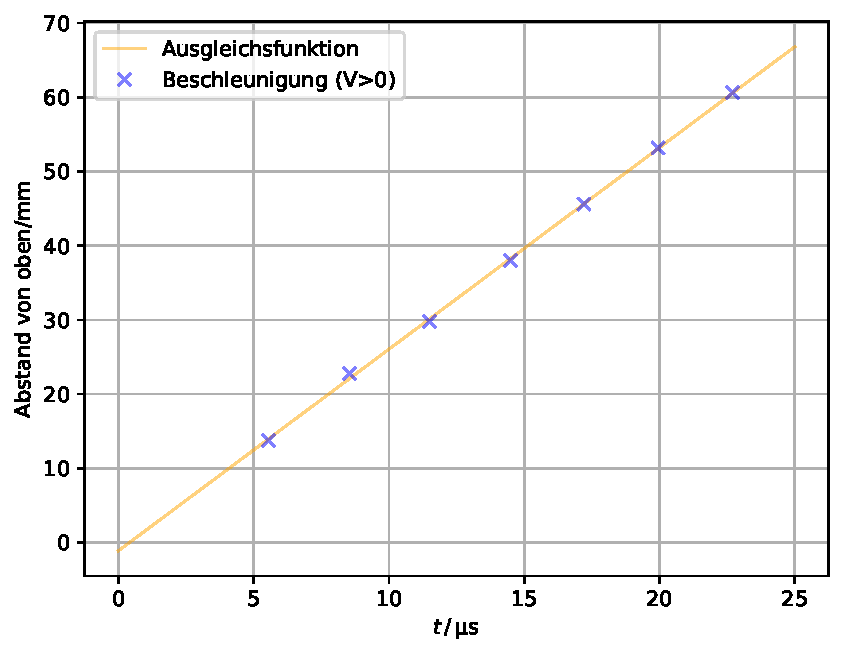
\includegraphics[height = 8cm]{build/plotv.pdf}
    \caption{Regression zur Bestimmung der Schallgeschwindigkeit und der Dicke der Anpassungsschicht.}
    \label{fig:plotv}
\end{figure}

Die Schichtdicke entspricht dem Betrag des y-Achsenabschnitt
\begin{equation*}
    d = \lvert b\rvert = \lvert (-1.1 \pm 0.4) \, \unit{\mm}\rvert =  (1.1 \pm 0.4) \, \unit{\mm} \& .
\end{equation*}
Die Schallgeschwindigkeit in Acryl ergibt sich über die Steigung der Ausgleichsgeraden
\begin{equation*}
    v = (2.718 \pm 0.025) \, \unit{\mm \per \micro\sec} = (2718\pm 25) \, \unit{\m\per\sec} \; .
\end{equation*}

\subsection{Untersuchung des Acrylblocks}
Die Messwerte des A-Scans von der oberen und unteren Seite des Acrylblocks befinden sich in \autoref{tab:AScan}. Dabei wurden die Tiefenmessungen 
mit der Schichtdicke korrigiert. Mithilfe der korrigierten Werte und der gemessenen Gesamthöhe des Blocks $h = 79.9\,\unit{\mm}$ ergibt sich über 
\begin{equation*}
    d = h - a_{\symup{ob}} - a_{\symup{unt}}
\end{equation*}
der Durchmesser der einzelnen Bohrungen, welcher ebenfalls in \autoref{tab:AScan} dargestllt ist.

\begin{table}
    \centering 
    \caption{Messwerte der Tiefe der einzelnen Bohrungen sowie dessen Durchmesser.}
\begin{tabular}{c c c c c c}
    \toprule
    Bohrung & Tiefe von oben in \unit{\mm} & Tiefe nach der Korrektur in \unit{\mm}& Tiefe von unten in \unit{\mm} & Tiefe nach der Korrektur in \unit{\mm} & Durchmesser d in \unit{\mm}\\
    \midrule
                        1&20.6&19.5&60.4&59.3&1.1 \\
                         2&19.0&17.9&62.0&60.9&1.1 \\
                         3&62.0&60.9&14.5&13.4&5.6 \\
                         4&54.5&53.4&23.0&21.9&4.6 \\
                         5&46.9&45.8&31.6&30.5&3.6 \\
                         6&39.5&38.4&40.1&39.0&2.5 \\
                         7&31.4&30.3&47.9&46.8&2.8 \\
                         8&23.3&22.2&56.0&54.9&2.8 \\
                         9&15.2&14.1&64.1&63.0&2.8 \\
                                     10&7.2&6.1&&& \\
                        11&55.8&54.7&16.8&15.7&9.5 \\
                        \bottomrule
    \end{tabular}
    \label{tab:AScan}
\end{table}
\section{Diskussion}
\label{sec:Diskussion}

Bei der Messung der Schallgeschwindigkeit kann der experimentelle Wert $v = (2718\pm 25) \, \unit{\m\per\s}$ mit dem theoretischen Wert 
$2700 \,\unit{\m\per\s}$ verglichen werden. Die experimentell bestimmte Schallgeschwindigkeit stimmt im Rahmen der Fehlerabweichung mit 
dem theoretischen Wert überein. Die Abweichung zwischen beiden Werten beträgt $0.6\,\%$. 

\subsection{Untersuchung des Acrylblocks mit einem A-Scan}
Sowohl die Werte des A-Scans als auch die Ergebnisse des B-Scans lassen sich mit den mit der Schieblehre ausgemessenen Werten sowie untereinander 
vergleichen.

Die Abweichungen des A-Scans zu den mit der Schieblehre gemessenen Werten sind in \autoref{tab:AAbweichung} dargestellt. 

\begin{table}
    \centering 
    \caption{Abweichungen zwischen dem A-Scan und den mit der Schieblehre bestimmten Werten.}
\begin{tabular}{c c c c}
    \toprule
    & \multicolumn{3}{c}{Abweichung der Messungen} \\
    Bohrung & von unten & von oben & Durchmesser\\
    \midrule
    1&0.5&1.6&35.3 \\
    2&0.3&2.3&35.3 \\
     3&1.5&0.5&6.7 \\
     4&0.9&0.4&8.0 \\
    5&1.7&0.4&10.0 \\
    6&1.0&1.1&16.7 \\
     7&0.4&1.7&7.7 \\
     8&0.4&2.6&7.7 \\
     9&0.5&2.9&7.7 \\
    10&5.9&--&-- \\
    11&2.6&0.6&4.0 \\
    \bottomrule
\end{tabular}
\label{tab:AAbweichung}
\end{table}
Dass die Messwerte nicht genau übereinstimmen, kann an ungenauen Messungen mit der Schieblehre sowie der Ungenauigkeit der Dicke der Anpassungsschicht 
liegen, die sich auf die Messergebnisse des A-Scans fortpflanzt.Die Abweichungen sind allgemein bei kleineren Messwerten größer, da bei einer kleinen 
Größenordnung der Messfehler mehr ins Gewicht fällt. Allgemein lässt sich sagen, dass die Messung mittels Ultraschall/A-Scan vermutlich genauere Ergebnisse 
liefert.

\newpage
\printbibliography
\nocite{apus1}
\nocite{matplotlib}
\nocite{numpy}
\nocite{scipy}
\nocite{uncertainties}
\nocite{reback2020pandas}

\newpage
%\includepdf[scale=0.7,pages=1,pagecommand=\section*{Anhang}\thispagestyle{empty}]{messdaten.pdf}
%\addcontentsline{toc}{section}{\protect\numberline{}Anhang}
%\includepdf[scale = 0.7, pages=-]{messdaten.pdf}

\end{document}
